\documentclass[journal]{IEEEtran}
\usepackage[a5paper, margin=10mm, onecolumn]{geometry}
\usepackage[cmex10]{amsmath}
\usepackage{amssymb,amsfonts,amsthm}
\usepackage{gvv-book}
\usepackage{gvv}
\usepackage{hyperref}

\begin{document}


\title{1.9.14}
\author{EE25BTECH11025 - Ganachari Vishwambhar}
\maketitle

\textbf{Question}:\newline
If $\vec{P}=\brak{2,2}$, $\vec{Q}=\brak{-4,-4}$, and $\vec{R}=\brak{5,-8}$ are the vertices of a triangle $\Delta PQR$, then find the length of the median through $\vec{R}$.\\
\textbf{Solution: }\\
Given position vectors of the points are:
\begin{align}
    \vec{P}=\myvec{2\\2},
    \vec{Q}=\myvec{-4\\-4},
    \vec{R}=\myvec{5\\-8}
\end{align}

Let the midpoint of vector $\vec{Q}-\vec{P}$ be $\vec{M}$:
\begin{align}
    \vec{M}=\frac{1}{2}\vec{P}+\frac{1}{2}\vec{Q}\\
    \vec{M}=\myvec{1\\1}+\myvec{-2\\-2}\\
    \vec{M}=\myvec{-1\\-1}\\
    \vec{M}-\vec{R}=\myvec{-1\\-1}-\myvec{5\\-8}\\
    \vec{M}-\vec{R}=\myvec{-6\\7}
\end{align}

The length of the median:
\begin{align}
    ||\vec{M}-\vec{R}||=\sqrt{\brak{-6}^2+\brak{7}^2}\\
    ||\vec{M}-\vec{R}||=\sqrt{85}\approx9.219
\end{align}

Thus the length of the median of the triangle through $\vec{R}$ is $\sqrt{85}\approx9.219$.

\begin{figure}[h!]
   \centering
   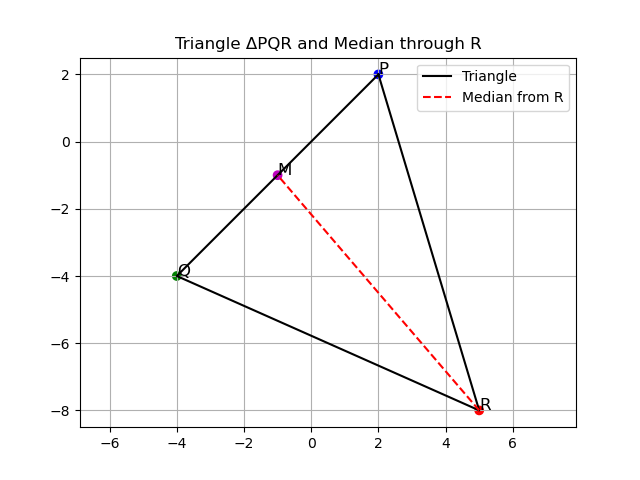
\includegraphics[width=0.7\linewidth]{figs/plot.png}
   \caption{Plot of line segment \textbf{AB}}
   \label{}
\end{figure}
\end{document}  
